\chapter[Experimentos y resultados]{Experimentos y resultados}\label{ch:capitulo5}
En este capítulo presentaremos los experimentos y los resultados obtenidos para la primera parte de este trabajo, que considera el estado del arte y la presentación del marco de desarrollo descrito en el Capítulo~\ref{ch:capitulo4}, el objetivo de este capítulo es discutir los resultados entregados por este marco de desarrollo con el objetivo de determinar sus ventajas y desventajas, para así tener una visión específica para los trabajos futuros. Además se presentan los trabajos futuros que discutiremos en la segunda parte de este trabajo.

\section{Experimentos}
Para esta primera etapa se utilizó el marco de desarrollo presentado en el Capítulo~\ref{ch:capitulo4}, con este marco de desarrollo creamos modelos para distintas categorías de objetos, ver Sección~\ref{subsec:m_obj}, objetos nuevos (Sección~\ref{subsec:m_new_im}), expresiones faciales (Sección~\ref{subsec:m_face}).

\subsection{Modelos para objetos}\label{subsec:m_obj}
Para la realización de este experimento creamos un modelo de predicción para botellas, latas, autos, aviones, bicicletas, etc. Utilizamos las imágenes pertenecientes a la base de imágenes de PASCAL, mencionada en el Capítulo~\ref{ch:capitulo4}, la que provee una cantidad de datos de entrenamiento considerablemente grande, aparte de entregarnos un sistema de anotaciones las cuales enmarcan a los objetos de interés para el proceso de entrenamiento y clasificación.

\subsection{Modelos para imágenes nuevas}\label{subsec:m_new_im}
El problema de la base de datos de imágenes de PASCAL es que no provee todo el universo de objetos que uno quisiera, esto nos da la oportunidad para que nosotros podamos agregar nuestros propios objetos y siguiendo el mismo procedimiento, poder crear las estructuras necesarias para que el marco de desarrollo cree los modelos correspondientes, por ejemplo, podemos agregar imágenes de latas, imágenes de cuadros, imágenes de estatuas.

\subsection{Modelos para expresiones faciales}\label{subsec:m_face}
Para las expresiones faciales, separamos estas expresiones en seis clases, correspondientes cada una de ellas a las expresiones canónicas, es decir, obtuvimos un conjunto de imágenes de entrenamiento para expresiones de alegría, asco, ira, miedo, sorpresa, tristeza. El objetivo es generar un modelo de predicción para cada una de estas expresiones.

\section{Resultados}
En esta sección presentaremos resultados obtenidos para la detección de botellas. Para este caso creamos un modelo de reconocimiento de botellas con el marco de desarrollo del Capítulo~\ref{ch:capitulo4}, luego con la imagen de prueba, Figura~\ref{fig:bottle}, comprobamos la efectividad del modelo. Los resultados obtenido para la Figura~\ref{fig:bottle}, se presentan en las Figuras~\ref{fig:bottle-parts},~\ref{fig:bottle-parts-final},~\ref{fig:bottle-final}.
\begin{figure}[tb]
\centering
 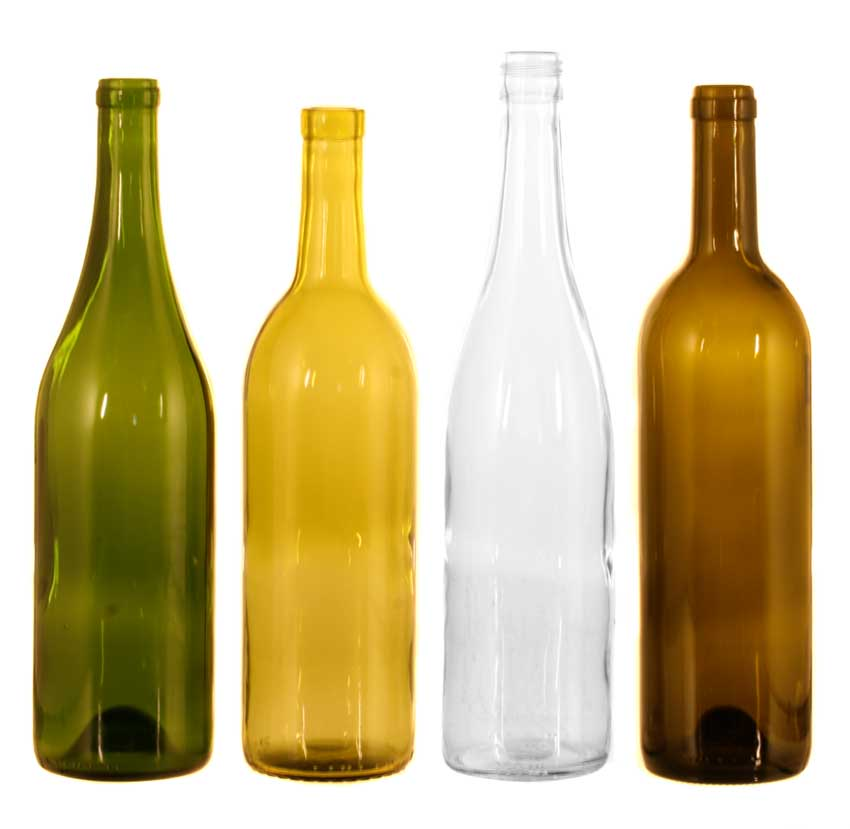
\includegraphics[width=0.6\textwidth]{Figuras/results/bottle.jpg}
 \caption[Imagen de botellas]{Imagen de prueba para categoría \textit{botella}, se espera poder detectar las cuatro botellas que hay presentes en la imagen.}
 \label{fig:bottle}
\end{figure}

\begin{figure}[tb]
\centering
 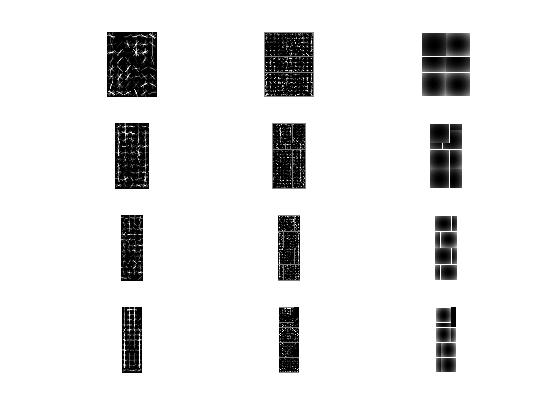
\includegraphics[width=0.8\textwidth]{Figuras/results/bottle-parts.jpg}
 \caption[Detección de partes para un objeto]{Detección de partes para Figura~\ref{fig:bottle}, en esta figura se muestran las partes obtenidas por el descriptor del marco de desarrollo, cabe destacar que el modelo fue entrenado con una pirámide con profundidad igual a cuatro.}
 \label{fig:bottle-parts}
\end{figure}

\begin{figure}[tb]
\centering
 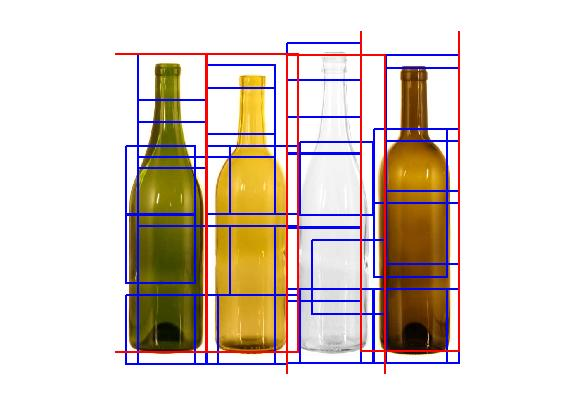
\includegraphics[width=0.8\textwidth]{Figuras/results/bottle-parts-final.jpg}
 \caption[Detección de partes en imagen de un objeto]{Detección de partes en Figura~\ref{fig:bottle}, de las partes extraídas por la pirámide se busca su mejor posición dentro de la imagen de prueba, además se presenta el filtro raíz. El objetivo de las partes es corroborar la posición del filtro raíz.}
 \label{fig:bottle-parts-final}
\end{figure}

\begin{figure}[tb]
\centering
 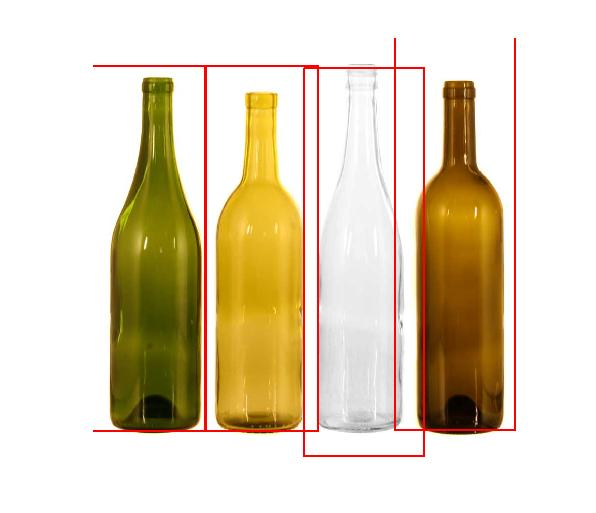
\includegraphics[width=0.8\textwidth]{Figuras/results/bottle-final.jpg}
 \caption[Detección final para un objeto]{Detección final para Figura~\ref{fig:bottle}, se eliminan las partes, y solo queda el filtro raíz ya que este último representa la mejor ventana de detección del objeto. Como se aprecia, las cuatro botellas de la imagen han sido detectadas.}
 \label{fig:bottle-final}
\end{figure}

Como se puede ver la detección es posible realizarla mediante la utilización de los modelos creados por el marco de desarrollo, en futuras entregas se probará su efectividad con otro tipo de descriptor, con el objetivo de generar una comparativa, para luego analizar la posibilidad de portar estos modelos a un sistema con menor potencia.
\section{Resumen}
En este capítulo se presentaron los experimentos realizados en esta etapa y algunos resultados obtenidos correspondientes al funcionamiento del marco de desarrollo descrito en el Capítulo~\ref{ch:capitulo4}. Podemos apreciar en la Figura~\ref{fig:bottle-final} que la detección de un objetos del tipo botella, ha sido posible mediante la creación de un modelo creado mediante la utilización de muchos datos de entrada que tenían precian de una botella, como se mencionó anteriormente estos datos son proporcionados por la base de imágenes de PASCAL. En el siguiente capítulo se presentan nuestras conclusiones sobre esta primera etapa del trabajo, además se presentan los trabajos pendiente y futuros que se realizarán en futuras entregas.


